\documentclass[11pt,aspectratio=169]{beamer}

% -------------------- THEME & LAYOUT --------------------
\usetheme{Madrid}
\usecolortheme{dolphin} % base color scheme
\usefonttheme{professionalfonts}
\setbeamercovered{transparent}
\setbeamertemplate{navigation symbols}{}   % remove navigation buttons
\setbeamertemplate{caption}[numbered]      % numbered captions
\setbeamertemplate{itemize items}[triangle]
\setbeamersize{text margin left=1.2cm,text margin right=1.2cm} % adjust to taste
% -------------------- GLOBAL FONT SETTINGS --------------------

% 1. Force the base beamer font to small
\setbeamerfont{normal text}{size=\small}

% 2. Force math environments to follow the "small" font size
\setbeamerfont{math text}{size=\small}
\setbeamerfont{equation}{size=\small}

% 3. Redefine \normalsize itself 
% This ensures equations and lists (which look for \normalsize) use  instead.
\let\oldnormalsize\normalsize
\renewcommand{\normalsize}{\oldnormalsize\small}

% 4. Ensure lists also stay small
\setbeamerfont{itemize/enumerate body}{size=\small}
\setbeamerfont{itemize/enumerate subbody}{size=\small}

% -------------------- FONTS & TYPOGRAPHY --------------------
\usepackage[T1]{fontenc}
\usepackage[utf8]{inputenc}
\usepackage{newpxtext,newpxmath} % Palatino-like font & math
\usepackage{microtype}

% -------------------- MATH, TABLES & GRAPHICS --------------------
\usepackage{amsmath,amssymb,amsfonts,mathtools}
\usepackage{bm,booktabs,siunitx,graphicx}
\graphicspath{{./}{./figures/}}
\renewcommand{\theequation}{5.\arabic{equation}}

% -------------------- UTILITIES --------------------
\usepackage{appendixnumberbeamer}
\usepackage{ragged2e}
\usepackage{xspace}
\usepackage{csquotes}
% -------------------- Bibliography --------------------
\usepackage[backend=biber,style=authoryear]{biblatex}
\addbibresource{sources.bib}
\usepackage{xcolor}

% -------------------- HYPERREF --------------------
\hypersetup{
  colorlinks=false,
  pdfauthor={Francesca},
  pdftitle={Chapter 1 — The Value of Currency}
}

% -------------------- COLORS & EMPHASIS --------------------
\definecolor{myblue}{RGB}{0,70,140}
\definecolor{myred}{RGB}{180,30,30}
\definecolor{mygreen}{RGB}{0,120,70}
\definecolor{gold}{RGB}{184,134,11}

\setbeamercolor{title}{fg=gold}       % title page
\setbeamercolor{frametitle}{fg=gold}  % slide titles
\setbeamercolor{structure}{fg=gold}   % bullets, sections, links
\setbeamercolor{section in head/foot}{fg=gold,bg=black!10} % gold text on light background

% -------------------- FOOTLINE --------------------
\setbeamertemplate{footline}{
  \leavevmode%
  \hbox{%
    % Section links (hidden if no current section)
    \begin{beamercolorbox}[wd=0.7\paperwidth,ht=2.5ex,dp=1.5ex,leftskip=1.4em]{section in head/foot}%
      \ifx\insertsection\empty
        % nothing
      \else
        Section: \insertsection
      \fi
    \end{beamercolorbox}%
    % Frame number right
    \begin{beamercolorbox}[wd=0.3\paperwidth,ht=2.5ex,dp=1.5ex,leftskip=3.8cm]{section in head/foot}%
      \insertframenumber/\inserttotalframenumber
    \end{beamercolorbox}%
  }%
  \vskip1pt%
}



\newcommand{\highlight}[1]{\textcolor{myblue}{#1}}
\newcommand{\warning}[1]{\textcolor{myred}{#1}}

% -------------------- SHORTCUTS --------------------
\newcommand{\E}{\mathbb{E}}
\newcommand{\R}{\mathbb{R}}
\newcommand{\dd}{\mathrm{d}}
\newcommand{\mc}[1]{\mathcal{#1}}
\newcommand{\bb}[1]{\mathbb{#1}}
\newcommand{\uc}{U_c}
\newcommand{\zg}{Z_g}

% -------------------- TIGHTER DISPLAY MATH --------------------
\makeatletter
\g@addto@macro\normalsize{%
  \setlength\abovedisplayskip{8pt}%
  \setlength\belowdisplayskip{8pt}%
  \setlength\abovedisplayshortskip{6pt}%
  \setlength\belowdisplayshortskip{6pt}%
}
\makeatother
\setbeamertemplate{frametitle}{
  \nointerlineskip
  \begin{beamercolorbox}[wd=\paperwidth,ht=3.5ex,dp=1ex,center]{frametitle}
    \centering\insertframetitle
  \end{beamercolorbox}
}

% -------------------- METADATA --------------------
\title[Part I — Currency and Money]{\textbf{Part I: Currency and Money}\\[2pt]\large Chapter 1 — The Value of Currency}
\subtitle{Currency, Money, and Price-Level Determination}
\author{Francesca}
\institute{}
\date{\today}

% -------------------- SECTION ROADMAP --------------------
\AtBeginSection[]
{
  \begin{frame}
    \tableofcontents[currentsection, hideothersubsections]
  \end{frame}
}


\begin{document}
\setcounter{equation}{0}


% ===================== TITLE SLIDE =====================
\begin{frame}[plain] % 'plain' removes header/footer for the title slide

\begin{columns}[T,totalwidth=\textwidth]

% ----- Left column: Main title, professor, chapter -----
\begin{column}{0.45\textwidth}
\vspace{2cm}

% Main title
{\usebeamercolor[fg]{title}\LARGE\textbf{Monetary Economics}\\[0.3cm]
\LARGE\textbf{and Policy}} 

\vspace{0.5cm}

% Professor name and date
{\large\textit{Pierpaolo Benigno}}\\[0.1cm]

\vspace{1cm}

% Chapter and subtitle
{\usebeamercolor[fg]{frametitle}\large Chapter 5: The Benchmark New Keynesian Model}

\end{column}

% ----- Right column: Image -----
\begin{column}{0.55\textwidth}
\vspace{1cm}
\centering
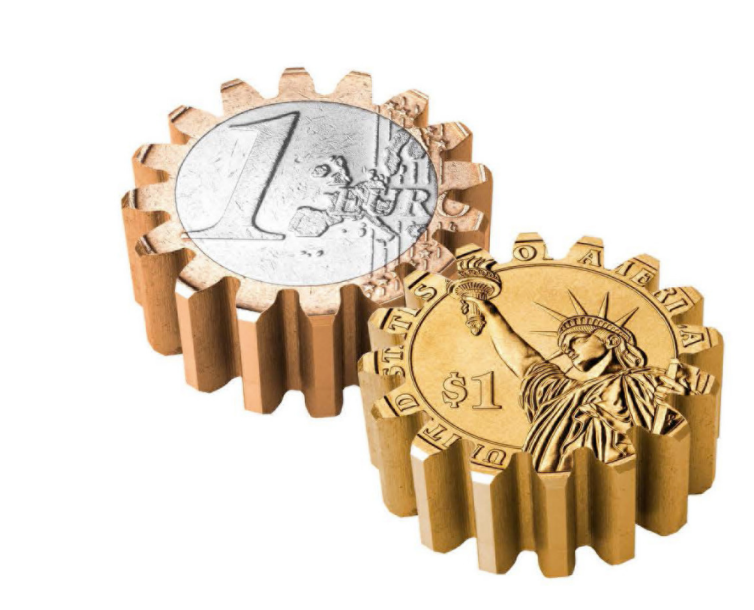
\includegraphics[width=0.9\linewidth]{Cover.png}
\end{column}

\end{columns}

% ----- Footer text (bottom-right corner) -----
\vspace*{2cm} % adjust if needed
\hfill{\large\textit{Prepared by Marcos Consuegra}}

\end{frame}


% --- INTRO SLIDE: What We Will Learn ---
\begin{frame}{What We Will Learn}
\small

\begin{itemize}
  \item How to extend the basic monetary framework by introducing 
        \textbf{nominal rigidities} through Calvo–Yun price setting.

  \item How price stickiness generates an \textbf{upward-sloping, 
        forward-looking aggregate supply (NKPC)} and a non-neutral role for monetary policy.

  \item How intertemporal optimization by households leads to a 
        \textbf{forward-looking aggregate demand (NK IS)} relation driven by the real interest rate.

  \item How to define and interpret the \textbf{natural rate of output} 
        and distinguish it from the \textbf{efficient level} of output.

  \item How to combine the NKPC and the NK IS equation into a 
        \textbf{log-linearized equilibrium system} describing short-run fluctuations.

  \item How monetary policy affects output and inflation through 
        both the \textbf{policy rate} and \textbf{expectation management}.
\end{itemize}

\end{frame}

% OUTLINE
\begin{frame}{Outline}
\tableofcontents
\end{frame}

\section{Introduction}

% --- SLIDE 1 ---
\begin{frame}{The Effectiveness of Monetary Policy}
\small


\begin{itemize}
  \item {\textcite{friedmanschwartz1963}}
is a statement on the importance of \textbf{stabilization policy} by central banks.

  \item Three key insights:
    \begin{itemize}
      \item \textbf{Natural rate of output}: long-run output is independent of monetary policy.
      \item \textbf{Short-run monetary non-neutrality}: 'transient' price rigidities allow monetary shocks to influence real activity.
      \item \textbf{Contractions and depressions}: major downturns are largely driven by contractions in the money supply.
    \end{itemize}

  \item \emph{“Prevention or moderation of the decline in the stock of money…  
          would have reduced the contraction’s severity and almost certainly its duration.” (\textcite{friedmanschwartz1963}, p. 301)}
\end{itemize}

\end{frame}

% --- SLIDE 2 ---
\begin{frame}{Limitations of Real Business Cycle Theories}
\small

\textbf{Real Business Cycle Models \parencite{kydlandprescott1982}}
\begin{itemize}
  \item Fully microfounded: households and firms solve intertemporal optimization under resource constraints.
  \item Incorporate stochastic technology shocks and rational expectations.
  \item Imply \textbf{monetary neutrality}—policy cannot affect real variables.
  \item Cannot account for the empirically observed short-run effects of monetary policy.
\end{itemize}

\vspace{0.2cm}

\textbf{Empirical Evidence: SVARs}
\begin{itemize}
  \item Monetary policy shocks stimulate output with a \textbf{lag of about six quarters}, with effects persisting for more than two years.
  \item These results provide empirical benchmarks for models of monetary transmission  
        \parencite{christiano1999, woodford2003}.
\end{itemize}

\end{frame}

\begin{frame}{Emergence of the New-Keynesian Theories}
\small

\begin{itemize}
  \item Builds on RBC \textbf{microfoundations}: intertemporal optimization, rational expectations, and stochastic disturbances.

  \item Introduces \textbf{nominal rigidities} through imperfect competition and sticky prices  
        \parencite{mankiw1985}.

  \item Reconciles:
    \begin{itemize}
      \item \textbf{Short-run monetary non-neutrality} (due to price stickiness).
      \item \textbf{Long-run natural rate of output} (as in RBC).
    \end{itemize}

  \item Provides a tractable framework consistent with SVAR evidence on the dynamic effects of monetary shocks.
\end{itemize}

\end{frame}

% --- SLIDE 5 ---
\begin{frame}{Nominal Rigidities}
\small

\begin{itemize}
  \item \textbf{Calvo–Yun price setting:} in each period, only a fraction $(1-\alpha)$ of firms can reset their price, while the remaining fraction keeps an indexed price.  
        This generates \textbf{staggered} price adjustments with random durations.

  \item Firms that reset understand that their price may remain fixed for several periods.  
        As a result, they choose prices \textbf{anticipating future inflation and marginal costs}.

  \item This forward-looking behavior yields an \textbf{upward-sloping aggregate supply (NK Phillips Curve)}, where inflation depends on:
    \begin{itemize}
      \item the current output gap, and  
      \item expected future inflation.
    \end{itemize}

  \item Sticky prices create the mechanism for \textbf{short-run monetary non-neutrality}:  
        by affecting real interest rates, monetary policy can influence output.
\end{itemize}

\end{frame}


% --- SLIDE 7 ---
\begin{frame}{Connecting Theory and Evidence}
\small

\begin{itemize}
  \item NKM bridges Friedman \& Schwartz’s empirical insights and RBC microfoundations.
  \item Captures realistic policy effects:
    \begin{itemize}
      \item Output responds gradually to monetary shocks.
      \item Inflation dynamics consistent with Calvo pricing.
    \end{itemize}
  \item Provides a framework for evaluating optimal monetary policy (e.g., inflation targeting).
\end{itemize}
\end{frame}

% --- SLIDE 8 ---
\begin{frame}{Limitations and Extensions}
\small

\begin{itemize}
  \item Benchmark NKM: single sector, time-dependent Calvo pricing, homogeneous shocks.
  \item Micro evidence shows heterogeneity and state-dependent price adjustment \parencite{nakamura2008, nakamura2013}.
  \item Calvo model remains a reasonable approximation for output response to a monetary shock.
  \item Extensions include banking sector, liquidity effects, and policy under financial crises (e.g., 2007–2008, COVID-19), which will be covered in later chapters.
\end{itemize}
\end{frame}

% --- SLIDE: Outline of the Chapter's Results ---
\begin{frame}{Outline of the Chapter’s Results}
\small

\textbf{Flexible Prices: Classical Benchmark}
\begin{itemize}
  \item With fully flexible prices, the model reproduces the \textbf{classical dichotomy}.
  \item Aggregate supply is \textbf{vertical}: shifts in aggregate demand affect only the price level, not output.
\end{itemize}

\vspace{0.15cm}

\textbf{Price Rigidities: New-Keynesian Benchmark}
\begin{itemize}
  \item Introducing \textbf{Calvo-style stickiness} yields an upward-sloping $AS$ curve.
  \item Monetary policy becomes \textbf{non-neutral in the short run} and can stabilize output.
\end{itemize}

\vspace{0.15cm}

\textbf{Forward-Looking Equations}
\begin{itemize}
  \item \textbf{Aggregate demand (NK IS):} output depends negatively on the \emph{current and expected future} real interest rate.
  \item \textbf{Aggregate supply (NKPC):} inflation depends on the \emph{present-discounted sum} of current and expected future output gaps.
  \item Monetary policy operates through the \textbf{policy rate} and by \textbf{shaping expectations}.
\end{itemize}

\end{frame}


\section{Model}

% --- SLIDE: Model Overview ---
\begin{frame}{Model Overview}
\small
\textbf{Stochastic Environment}
\begin{itemize}
  \item Infinite-horizon, closed economy with uncertainty.
  \item The state of nature at time $t$ is denoted by $s_t \in \mc{S}$, where the set $\mc{S}$ is invariant over time.
  \item The history up to time $t$ is $s^{t} \equiv (s_t, s_{t-1}, \dots, s_{t_0})$.
  \item The probability distribution of histories is given by $f(s^{t}\mid s_{t_0})$ and has the Markov properties.
\end{itemize}

\textbf{Agents}
\begin{itemize}
  \item Households
  \item Firms
  \item Government
\end{itemize}
\end{frame}

\begin{frame}{Households: Preferences and Consumption}
\small
\textbf{Expected Intertemporal Utility}
\begin{equation}
E_{t_{0}}\left\{ \sum_{t=t_{0}}^{\infty }\beta ^{t-t_{0}}\xi _{t}\left[
U(C_{t})-\int_{0}^{1}H(L_{t}(j))dj\right] \right\}.  \label{UtilityNK}
\end{equation}

\textbf{Interpretation}
\begin{itemize}
\item $\beta \in (0,1)$: subjective discount factor
\item $\xi_t$: preference shock
\item $U(\cdot)$: concave utility in a consumption bundle $C$
\item $H(\cdot)$: convex disutility from hours of labor, supplied to firms producing good $j$. 
\end{itemize}
\end{frame}
% --- SLIDE 2: Consumption Aggregation ---
\begin{frame}{Household: Consumption Bundle}
\small
\textbf{Dixit–Stiglitz Aggregator}
\begin{equation}
C_{t}=\left[ \int_{0}^{1} C_{t}(j)^{\frac{\theta -1}{\theta}}, dj \right]^{\frac{\theta}{\theta -1}},
\qquad \theta > 1.
\label{DSaggregator}
\end{equation}

\textbf{Interpretation}
\begin{itemize}
\item $C_t(j)$: consumption of variety $j \in [0,1]$
\item $\theta$: elasticity of substitution across goods
\item Higher $\theta$ $\Rightarrow$ goods more substitutable
\item $\theta \to \infty$: perfect substitutes $\Rightarrow C_t = \int_0^1 C_t(j), dj$
\end{itemize}
\end{frame}

% --- SLIDE 3: Demand and Price Index ---
\begin{frame}[label=Aggregators]{Household: Demand of Goods}
\small
\textbf{Demand for Variety $j$}
\begin{equation}
C_{t}(j)=\left(\frac{P_{t}(j)}{P_{t}}\right)^{-\theta}C_{t}.
\label{DemandC}
\end{equation}
\vspace{0.45cm}

\begin{itemize} \item Demand depends on the relative price of good $j$, $P_t(j)$, with respect to the aggregate price index $P_t$:
\end{itemize}
\vspace{0.4cm}
\textbf{Aggregate Price Index}
\begin{equation}
P_{t}=\left[\int_{0}^{1} P_{t}(j)^{1-\theta}\,dj\right]^{\!\frac{1}{1-\theta}}.
\label{Pindex}
\end{equation}

\vspace{0.4cm}
\begin{center}
\hyperlink{Appendix D}{\beamerbutton{Derivation of demand and price index in Appendix}}
\end{center}
\end{frame}

% --- SLIDE 4: Complete Financial Markets ---
\begin{frame}{Households: Consumption, Saving, and Labor Supply}
\small
\textbf{Optimization Problem}
\begin{itemize}
\item At each point in time and contingencies, households choose consumption, saving, and hours worked.

\item They plan savings using available assets to smooth consumption across future states.

\item Financial markets are assumed to be \textbf{complete}, allowing the households to implement arbitrary patterns of portfolio payoffs across successor states.
\end{itemize}
\end{frame}

\begin{frame}{Complete Financial Markets}
\small
\textbf{Complete Markets}
\begin{itemize}
\item Denote $\mathcal{W}_t(s_{t+1})$ as the desired random payoff in state $s_{t+1}$ at $t+1$, conditional on history $s^t$.
\item Complete markets mean any desired random payoff $\mathcal{W}_t(s_{t+1})$ can be replicated by portfolios.
\item Number of traded assets $\geq$ number of possible states at $t+1$.
\item No-arbitrage: portfolios with identical payoffs have identical prices.
\end{itemize}
\end{frame}


\begin{frame}{Complete Financial Markets}
\small
    \textbf{Complete markets can be characterized by a set of state-contingent securities spanning all states of nature:}
\begin{itemize}
    \item A state-contingent security, at time $t$, pays 1 unit of currency in a specific state $s_{t+1}$ at date $t+1$, and 0 otherwise.
    \item Price of the security at $t$: $\dfrac{v_t(s_{t+1})}{1+i_t}$, conditional on history $s^t$.
    \item Note: Normalization by $(1+i_t)$ is for analytical convenience; $i_t$ is the nominal risk-free rate.
\end{itemize}
\end{frame}

% --- SLIDE 1: From State Prices to Portfolio Valuation ---
\begin{frame}{Portfolio Valuation under Complete Markets}
\small
\begin{itemize}
    \item A generic portfolio with random payoff $\mathcal{W}_{t+1}$ has value:
    \[
    B_t = \sum_{s_{t+1} \in S} \frac{v_t(s_{t+1})}{1+i_t}\,\mathcal{W}_t(s_{t+1}).
    \]
    \item Each payoff $\mathcal{W}_{t+1}$ is valued through the price of the respective state-contingent security, $\frac{v_t(s_{t+1})}{1+i_t}$.
    \item No-arbitrage implies identical prices for portfolios with identical payoffs.
\end{itemize}
\textbf{Stochastic Discount Factor (SDF)}
    \[
    \tilde{R}_{t}(s_{t+1}) \equiv \frac{v_t(s_{t+1})}{f_t(s_{t+1})(1+i_t)},
    \]
    \hspace{0.65cm}where $f_t(s_{t+1}) \equiv f_t(s_{t+1}|s^t)$.
\end{frame}

\begin{frame}{Portfolio Valuation under Complete Markets}
\small
\begin{itemize}
    \item Using the stochastic discount factor into the valuation of the portfolio:
\end{itemize}
\begin{eqnarray}
B_{t} &=&\sum_{s_{t+1}\in S}f_{t}(s_{t+1})\tilde{R}_{t}(s_{t+1})\mathcal{W}%
_{t}(s_{t+1})\notag \\
&=&E_{t}\tilde{R}_{t,t+1}\mathcal{W}_{t+1}. \label{Port_Value}
\end{eqnarray}%
\textbf{Interpretation}
\begin{itemize}
    \item The price of a portfolio with a random return $\mathcal{W}_{t+1}$ is equal to the expected discounted value of its payoff, where the discount factor is represented by the random variable $\tilde{R}_{t,t+1}\equiv \tilde{R}_{t}(s_{t+1})$. 
    \item Note: For simplicity,  $\mathcal{W}_{t+1}$ is used in place of $\mathcal{W}_{t,t+1}$.
\end{itemize}
\end{frame}

% --- SLIDE 4: Risk-Free Bond and the SDF ---
\begin{frame}{Risk-Free Bond and the Stochastic Discount Factor}
\small
\textbf{Risk-Free Portfolio}
\begin{itemize}
    \item Consider a risk-free portfolio paying $\mathcal{W}_t(s_{t+1}) = 1$ for each $s_{t+1}\in\mathcal{S}$, the portfolio replicates the price of a risk-free nominal bond $B_t = \frac{1}{1+i_t}$.
\item Using \eqref{Port_Value}:
\[
\frac{1}{1+i_t} = E_t[\tilde{R}_{t,t+1}],
\]
implies for state-contingent prices:
\[
\sum_{s_{t+1} \in S} v_t(s_{t+1}) = 1.
\]
    \item The sum of state-contingent security prices equals one, consistent with no-arbitrage.
\end{itemize}
\end{frame}
% --- SLIDE 5: Household Budget Constraint ---
\begin{frame}{Household: Flow Budget Constraint}
\small
\textbf{Budget Constraint at time $t$}
\begin{equation}
\underbrace{B_t + P_t C_t}_{\text{total spending}} = \underbrace{\mathcal{W}_t + \int_0^1 W_t(j)L_t(j)dj + \Psi_t - T_t}_{\text{total resources net of taxes}}
\label{eq:household_bc}
\end{equation}

\textbf{Interpretation}
\begin{itemize}
    \item $B_t$: value of the portfolio with state-contingent payoffs $\mathcal{W}_{t+1}$.
    \item $P_t C_t$: nominal consumption spending .
    \item $\mathcal{W}_t$: payoff from past portfolio holdings.
    \item $\int_0^1 W_t(j)L_t(j)dj$: income from each variety of labor $j$ supplied.
    \item $\Psi_t$: firms’ profits
    \item $T_t$: Taxes.
    \item Note: Cash is neglected, since it is only held at $i_t = 0$, imposing a ZLB.
\end{itemize}
\end{frame}

\begin{frame}{Household: Borrowing Limit Condition}
\small

\vspace{0.3cm}
\noindent\textbf{Borrowing Limit:}
\begin{equation*}
-\mathcal{W}_{t}\leq E_{t}\left\{ \sum_{T=t}^{\infty }\tilde{R}%
_{t,T}(W_{T}L_{T}+\Psi _{T}-T_{T})\right\} <\infty ,
\end{equation*}%
\hspace{0.65cm}
\vspace{0.45cm}
for each time $t\geq t_{0}$ and contingency at time $t;$ \textbf{or}, alternatively:     

\vspace{0.3cm}
\textbf{Intertemporal Budget Constraint:}
\begin{equation}
\underbrace{E_{t}\left\{ \sum_{T=t}^{\infty }\tilde{R}_{t,T}(P_{T}C_{T})\right\}}_\text{Expected PDV of Consumption} \leq 
\underbrace{\mathcal{W}_{t}+E_{t}\left\{ \sum_{T=t}^{\infty }\tilde{R}%
_{t,T}(W_{T}L_{T}+\Psi _{T}-T_{T})\right\}}_\text{Porfolio Payoff and PDV of Net Income}.  \label{IBCch6}
\end{equation}%
\end{frame}
\begin{frame}{Representative Consumer: Optimization Problem}
\small
\begin{itemize}
    \item The representative consumer chooses stochastic sequences 
$\{C_t, \mathcal{W}_{t+1}, L_t\}_{t=t_0}^\infty$ 
to maximize expected intertemporal utility:
\end{itemize}
\[
E_{t_{0}}\left\{ \sum_{t=t_{0}}^{\infty }\beta ^{t-t_{0}}\xi _{t}\left[
U(C_{t})-\int_{0}^{1}H(L_{t}(j))dj\right] \right\}.
\]

\textbf{Subject to:}
\begin{itemize}
  \item Portfolio valuation \eqref{Port_Value}
  \item Budget constraint \eqref{eq:household_bc}
  \item Intertemporal budget constraint \eqref{IBCch6}
  \item Non-negativity constraints $C_t, L_t \ge 0$
  \item Given initial condition 
  $\mathcal{W}_{t_0}$
\end{itemize}
\end{frame}

% --- SLIDE: Household Optimality Conditions ---
\begin{frame}[label=household_opt]{Household Optimality: Euler Equation}
\small

\begin{itemize}
  \item The following first-order condition characterizes the representative household’s optimal consumption/saving choice at time $t$:
\end{itemize}
\vspace{0.3cm}
\textbf{Euler Equation}
\begin{equation}
\frac{\xi_t \, U_c(C_t)}{P_t} = 
\frac{\beta}{\tilde{R}_{t,t+1}} \frac{\xi_{t+1} \, U_c(C_{t+1})}{P_{t+1}}.
\label{EulerCont}
\end{equation}

\begin{itemize}
  \item $U_c(\cdot)$ is the marginal utility of consumption.
  \item For each state at $t+1$, there is a corresponding Euler equation.
  \item Complete markets allow households to allocate consumption optimally across all contingencies at $t+1$.
\end{itemize}
\end{frame}

% --- SLIDE: Euler Equation with State-Contingent Securities ---
\begin{frame}[label=EulerStates]{Household Optimality: Euler Equation}
\small

\begin{itemize}
  \item The Euler equations can be expressed in terms of state-contingent securities as:
\end{itemize}

\vspace{0.3cm}
\begin{equation}
\underbrace{\frac{v_{t}(s_{t+1})}{1+i_t} \frac{\xi_t U_c(C_t)}{P_t}}_{\substack{\text{\scriptsize marginal cost of saving} \\ \text{\scriptsize one unit today, delivering one } \\ \text{\scriptsize unit of currency in state } s_{t+1}}}
=
\underbrace{\beta \, f_t(s_{t+1}) \frac{\xi_{t+1} U_c(C_{t+1})}{P_{t+1}}}_{\substack{\text{\scriptsize discounted marginal benefit of } \\ \text{\scriptsize consuming one unit tomorrow} \\ \text{\scriptsize in state } s_{t+1}}}.
\label{EulerStateContingent}
\end{equation}

\begin{itemize}
  \item The benefit is positive with probability $f_t(s_{t+1})$.
\end{itemize}

\end{frame}

% --- SLIDE: Stochastic Euler Equation ---
\begin{frame}[label=StochasticEuler]{Household Optimality: Stochastic Euler Equation}
\small

\begin{itemize}
  \item Multiplying \eqref{EulerCont} by $\tilde{R}_{t,t+1}$ and taking expectations at time $t$ yields:
\end{itemize}
\vspace{0.3cm}
\textbf{Stochastic Euler Equation}
\begin{equation}
\xi_t U_c(C_t)
=
\beta (1+i_t) E_t\left\{\frac{P_t}{P_{t+1}} \xi_{t+1} U_c(C_{t+1}) \right\}.
\label{SEuler}
\end{equation}

\vspace{0.2cm}
\begin{itemize}
  \item Having used $E_t \tilde{R}_{t,t+1} = 1/(1+i_t)$.
  \item \textbf{Note:} (\ref{SEuler}) is implied by the full set of state-contingent Euler equations \eqref{EulerCont}, but it does \emph{not} imply them.
\end{itemize}

\end{frame}

% --- SLIDE: Labor Supply ---
\begin{frame}[label=LaborSupply]{Household Optimality: Labor Supply}
\small

\textbf{Optimal Labor Supply for each variety of labor $j\in[0,1]$}
\vspace{0.3cm}
\begin{equation}
\underbrace{\frac{H_{l}(L_{t}(j))}{U_{c}(C_{t})}}_{\text{\scriptsize Marginal Rate of Substitution}}
=
\underbrace{\frac{W_t(j)}{P_t}}_{\text{\scriptsize Real Wage for variety $j$}}
\label{LaborSupply}
\end{equation}

\vspace{0.25cm}
\begin{itemize}
  \item $H_l(\cdot)$ denotes the derivative of disutility of labor with respect to hours supplied.
  \item Concavity of $U(\cdot)$ and convexity of $H(\cdot)$ imply labor supply is increasing in the real wage and decreasing in consumption.
  \item At the optimum, the intertemporal budget constraint \eqref{IBCch6} holds with equality at all times and in all states.
\end{itemize}

\end{frame}

% Firms
% --- SLIDE 2: Market Structure ---
\begin{frame}[label=FirmMarket]{Firms: Market Structure and Pricing Power}
\small

\begin{itemize}
  \item Firms operate in a market characterized by \textbf{monopolistic competition}: goods are differentiated, not perfect substitutes.
  \vspace{0.5em}
  \item Each firm can influence its demand by setting $P_t(j)$ through the demand function \eqref{Demand}.
\vspace{0.5em}
\item Firms are \emph{small} relative to the overall market, taking aggregate price $P_t$ and quantities $(C_t, G_t)$ as given.
\end{itemize}

\end{frame}
% --- SLIDE: Firms and Production ---
\begin{frame}[label=Firms]{Firms: Demand and Technology}
\small
\begin{itemize}
    \item Aggregate demand for firm $j$ depends on both private demand $C_t(j)$ and government demand $G_t(j)$:
\end{itemize}
\textbf{Demand for Firm $j$'s Output}
\begin{equation}
Y_t(j) = C_t(j) + G_t(j) = \left(\frac{P_t(j)}{P_t}\right)^{-\theta} (C_t + G_t).
\label{Demand}
\end{equation}

\begin{itemize}
  \item Assuming similar demand of $G$, i.e., $G_t(j) = \left(P_t(j)/P_t\right)^{-\theta} G_t$.
\end{itemize}

\vspace{0.3cm}
\textbf{Production Technology}
\begin{equation}
Y_t(j) = A_t L_t(j)
\end{equation}

\begin{itemize}
  \item $A_t$: stochastic labor productivity shock, identical across firms.
\end{itemize}

\end{frame}
% --- SLIDE 1: Firm Profits ---
\begin{frame}[label=FirmProfits]{Firms: Profits}
\small

\textbf{Profit Function for Firm $j$}
\vspace{0.2cm}
\begin{eqnarray}
\Psi_t(j) &=& (1+\tau_t^s) P_t(j) Y_t(j) - W_t(j) L_t(j) \notag \\
&=& \left[ (1+\tau_t^s) P_t(j) - \frac{W_t(j)}{A_t} \right] Y_t(j),
\label{Profits}
\end{eqnarray}

\begin{itemize}
  \item $\tau_t^s$: stochastic revenue subsidy.
  \item Note: The subsidy is useful to introduce a stochastic markup shifter and ensure an efficient steady-state equilibrium (simplifying the analysis of optimal policy in Chapter 7).
\end{itemize}

\end{frame}


% --- SLIDE: Government Budget Constraint ---
\begin{frame}[label=Government]{Government: Consolidated Budget Constraint}
\small

\textbf{Government Budget Constraint}
\vspace{0.2cm}
\begin{eqnarray}
B_t^g &=& (1+i_{t-1}) B_{t-1}^g + \int_0^1 P_t(j) G_t(j) \, dj + 
\tau_t^s \int_0^1 P_t(j) Y_t(j) \, dj - T_t \notag \\
&=& (1+i_{t-1}) B_{t-1}^g + P_t G_t + \tau_t^s P_t Y_t - T_t.
\label{BCTreasury2}
\end{eqnarray}

\begin{itemize}
  \item $B_t^g$: government debt; $T_t$: lump-sum taxes.  
  \item $P_t G_t$: nominal government spending; $\tau_t^s P_t Y_t$: subsidy to all firms.  
  \item Second line uses $G_t(j) = (P_t(j)/P_t)^{-\theta} G_t$, $Y_t(j) = (P_t(j)/P_t)^{-\theta} Y_t$, and the aggregate price index \eqref{Pindex}.  
  \item The central bank backs treasury debt, i.e., government debt is unconstrained by solvency conditions (see Chapter 1).
\end{itemize}

\end{frame}

% --- SECTION: Equilibrium with Flexible Prices ---
\section{Equilibrium with Flexible Prices\label{CH5-Flex}}

% --- SLIDE: Flexible Price Equilibrium ---
\begin{frame}[label=FlexEquilibrium]{Equilibrium: Flexible Prices}
\small

\begin{itemize}
  \item With flexible prices, each firm $j$ sets $P_t(j)$ to maximize profits \eqref{Profits} given demand \eqref{Demand}:
\end{itemize}

\textbf{Optimal Pricing Rule}
\begin{equation*}
P_t(j) = \underbrace{\mu_t \frac{W_t(j)}{A_t},}_{\substack{\text{Markup over} \\ \text{nominal marginal cost}}}
\quad 
\mu_t \equiv \frac{1}{1+\tau_t^s} \frac{\theta}{\theta-1}
\end{equation*}
\begin{itemize}
  \item Rewriting, we note that firm $j$'s labor demand is flat at the real wage:
\end{itemize}
\textbf{Labor Demand}
\begin{equation*}
\frac{W_t(j)}{P_t(j)} = \frac{A_t}{\mu_t}, \quad \text{constant across all } j.
\end{equation*}
\begin{center}
\hyperlink{Appendix D.2}{\beamerbutton{Derivation of Optimal Pricing Rule in Appendix}}
\end{center}
\end{frame}

% --- SLIDE: Labor Demand and Price Equalization ---
\begin{frame}[label=LaborEquilibrium]{Equilibrium: Labor and Prices}
\small

\begin{itemize}
  \item Household labor supply \eqref{LaborSupply} combined with firm labor demand yields:
\end{itemize}
\begin{equation*}
\frac{H_l(L_t(j))}{U_c(C_t)} = \frac{A_t}{\mu_t}\frac{P_t(j)}{P_t}, \quad \forall j
\end{equation*}

\begin{itemize}
  \item Convexity of $H(\cdot)$ implies a symmetric equilibrium:
  \begin{itemize}
      \item Labor is identical across firms: $L_t(j) = L_t$.
      \item Output is equal across goods: $Y_t(j) = Y_t$.
      \item Prices are uniform across goods: $P_t(j) = P_t$.
  \end{itemize}
\end{itemize}

\end{frame}

% --- SLIDE: Natural Rate of Output ---
\begin{frame}[label=NaturalOutput]{Equilibrium: Natural Rate of Output}
\small

\begin{itemize}
  \item Substituting $L_t = Y_t / A_t$ and using goods market equilibrium $C_t = Y_t - G_t$ gives:
\end{itemize}
\textbf{Natural Level of Output $Y_t^n$}

\begin{equation}
\frac{H_l\left(\frac{Y_t^n}{A_t}\right)}{U_c(Y_t^n - G_t)} = \frac{A_t}{\mu_t}.
\label{YNatural}
\end{equation}
\textbf{ Properties:}
\begin{itemize}
  \item $Y_t^n \uparrow$ in $A_t$ and $G_t$; $Y_t^n \downarrow$ in $\mu_t$.
  \item Higher productivity → firms hire more labor → output rises.
  \item Higher government spending → positive wealth effect → labor supply and output rise, but consumption falls.
  \item Higher markup → labor demand falls → output falls. 
\end{itemize}

\end{frame}

% --- SLIDE: Classical Dichotomy ---
\begin{frame}[label=ClassicalDichotomy]{Flexible-Price Equilibrium}
\small

\begin{itemize}
  \item \textbf{Classical Dichotomy:} Equation \eqref{YNatural} implies that in the flexible-price equilibrium, the real allocation is independent of monetary policy.
  \vspace{0.5em}
  \item Monetary policy \textbf{does} influence nominal variables such as interest rates and prices.
  \vspace{0.5em}
  \item The analysis from Chapter 1 applies, with the caveat that the economy is stochastic and output is now endogenously determined.
\end{itemize}

\end{frame}

% --- SLIDE: Efficient Output vs Natural Output ---
\begin{frame}[label=EfficientOutput]{Efficient vs. Natural Output}
\small

\begin{itemize}
  \item Assume the central planner chooses $Y_t$ to maximize consumer utility \eqref{UtilityNK} subject to the resource constraint $Y_t = C_t + G_t$ and production technology $Y_t = A_t L_t$ implies:
\end{itemize}
\textbf{Efficient Level of Output $Y_t^e$}
\begin{equation}
\frac{H_\ell\!\left(\frac{Y_t^e}{A_t}\right)}{U_c(Y_t^e - G_t)} = A_t.
\label{YEfficient}
\end{equation}

\begin{itemize}
  \item Comparing \eqref{YNatural} and \eqref{YEfficient}:
  \begin{itemize}
    \item \textbf{Markup shock} $\rightarrow$ \textbf{inefficient shock} (affect $Y_t^n$ but not $Y_t^e$).
    \item \textbf{Productivity \& government spending shock} $\rightarrow$ \textbf{efficient shocks} (affect $Y_t^n$ and $Y_t^e$ in the same proportion).
  \end{itemize}
\end{itemize}

\end{frame}

\section{Price Rigidities}
% --- SLIDE: Introduction to Price Rigidities ---
\begin{frame}[label=PriceRigidities]{Price Rigidities: Calvo Pricing}
\small

\begin{itemize}
  \item \textbf{Monetary policy neutrality} can be broken by introducing \textbf{price rigidities}.
  \item Benchmark mechanism: \textbf{\textcite{calvo1983} / \textcite{yun1996}}.
  \end{itemize}
  \textbf{Setup}
  \begin{itemize}
  \item Continuum of firms $j \in [0,1]$; each period, a fraction \textbf{$(1-\alpha)$} can reset their price.
  \item A price set at time $t$ remains for next period $t+1$ with probability \textbf{$\alpha$}, and for period $T>t$ with probability \textbf{$\alpha^{T-t}$}.
  \item \textbf{Non-reset prices} are indexed to the inflation target $\Pi$: if $P_t(j)$ persists until $T$, then \textbf{$P_T(j) = P_t(j) \Pi^{T-t}$}.
  \item Adjusting firms choose prices to maximize the \textbf{expected discounted value of profits}, taking into account the probability of the price remaining ---appropriately indexed.
\end{itemize}

\end{frame}

% --- SLIDE: Profits under Calvo Pricing ---
\begin{frame}[label=CalvoProfits]{Price Rigidities: Profits}
\small

\textbf{Profits at $T>t$ conditional on the price chosen at time $t$}
\begin{eqnarray*}
\Psi_T(j) &=& (1+\tau_T^s) P_t(j) \Pi^{T-t} Y_T(j) - W_T(j) L_T(j) \\
&=& (1+\tau_T^s) P_t(j) \Pi^{T-t} Y_T(j) - \frac{W_T(j)}{A_T} Y_T(j)
\end{eqnarray*}

Having used the production function: $L_T(j) = Y_T(j)/A_T$.
\break

\textbf{Demand at time $T$ conditional on price set at $t$:}
\begin{equation}
    Y_T(j) = \left(\frac{P_t(j) \Pi^{T-t}}{P_T}\right)^{-\theta} Y_T \label{DemandCalvo}
\end{equation}
\end{frame}

% --- SLIDE: Expected Discounted Profits ---
\begin{frame}[label=CalvoExpectedProfits]{Price Rigidities: Optimization Problem}
\small

\textbf{Expected present-discounted value of profits} for a firm $j$ that has set prices at time $t$

\begin{equation}
E_t \sum_{T=t}^{\infty} \alpha^{T-t} \tilde{R}_{t,T} 
\Big[ (1+\tau_T^s) \Pi^{T-t} P_t(j) Y_T(j) - \frac{W_T(j)}{A_T} Y_T(j) \Big].
\label{ProfitsValco}
\end{equation}

\begin{itemize}
  \item Firm $j$ chooses $P_t(j)$ to maximize (\ref{ProfitsValco}) given demand \eqref{DemandCalvo}.
  \item \textbf{Note:} Wages $W_T(j)$ are taken as given (firms are small in their sector, wage-takers).
\end{itemize}
\end{frame}

% --- SLIDE: Optimal Price under Calvo Pricing ---
\begin{frame}[label=CalvoOptimalPrice]{Price Rigidities: Optimality Condition}
\small

\textbf{First-order condition for optimal price $P_t(j)$:}

\begin{equation}
\frac{P_t(j)}{P_t} = 
\frac{
E_t \left\{ \sum_{T=t}^{\infty} (\alpha \beta)^{T-t} \xi_T U_c(C_T) 
\left( \frac{P_T}{P_t} \frac{1}{\Pi^{T-t}} \right)^\theta 
\frac{W_T(j)}{A_T P_T} Y_T \right\}
}{
E_t \left\{ \sum_{T=t}^{\infty} (\alpha \beta)^{T-t} \xi_T U_c(C_T) 
\left( \frac{P_T}{P_t} \frac{1}{\Pi^{T-t}} \right)^{\theta-1} 
\frac{Y_T}{\mu_T} \right\}
}.
\label{ASn11}
\end{equation}

\begin{itemize}
  \item Discount factor: $\tilde{R}_{t,T} = \beta^{T-t} \frac{\xi_T U_c(C_T)}{\xi_t U_c(C_t)} \frac{P_t}{P_T}$ using \eqref{EulerCont}.
  \item Recall, $\mu_t = \theta / [(1+\tau_t^s)(\theta-1)]$.
  \item In equilibrium, all adjusting firms set $P_t(j) = \mathcal{P}_t^\ast$.
  \item Uniqueness is ensured because the LHS increases in $P_t(j)$ and the RHS decreases due to dependence of $W_T(j)$ on $P_t(j)$.
\end{itemize}

\end{frame}

% --- SLIDE: Calvo Pricing with Isoelastic Labor ---
\begin{frame}[label=CalvoIsoelastic]{Price Rigidities: Optimality Condition}
\small

\begin{itemize}
  \item Assume isoelastic disutility of labor:
\end{itemize}

\begin{equation*}
H(L(j)) = \frac{L(j)^{1+\eta}}{1+\eta}, \quad \eta \ge 0 \text{ (Frisch elasticity).}
\end{equation*}

\begin{itemize}
  \item Using \eqref{LaborSupply}, $L_T(j)=Y_T(j)/A_T$ and \eqref{DemandCalvo}, we can substitute $W_T(j)/P_T$ in \eqref{ASn11} to simplify the optimal price condition:
\end{itemize}
\vspace{0.5em}
\textbf{Optimal Price with Isoelastic Labor Disutility}

\begin{equation}
\left( \frac{\mathcal{P}_t^\ast}{P_t} \right)^{1+\theta \eta} = 
\frac{
E_t \Big\{ \sum_{T=t}^{\infty} (\alpha \beta)^{T-t} \xi_T 
\left( \frac{P_T}{P_t} \frac{1}{\Pi^{T-t}} \right)^{\theta(1+\eta)} 
\left( \frac{Y_T}{A_T} \right)^{1+\eta} \Big\}
}{
E_t \Big\{ \sum_{T=t}^{\infty} (\alpha \beta)^{T-t} \xi_T U_c(C_T) 
\left( \frac{P_T}{P_t} \frac{1}{\Pi^{T-t}} \right)^{\theta-1} 
\frac{Y_T}{\mu_T} \Big\}
}.
\label{ASn33}
\end{equation}

\end{frame}

% --- SLIDE: Law of Motion for the Price Index ---
\begin{frame}[label=CalvoPriceIndex]{Price Rigidities: General Price Index}
\small

\begin{itemize}
    \item   Remaining fraction $\alpha$ of firms (not adjusting) index their previous prices to the inflation target $\Pi$.
    \vspace{0.5em}
  \item Using the law of large numbers, recursive aggregation of all past price vintages implies:
\end{itemize}

\textbf{Law of Motion for the Aggregate Price Index:}
\begin{equation}
P_t^{1-\theta} = (1-\alpha) (\mathcal{P}_t^\ast)^{1-\theta} + 
\alpha \, \Pi^{1-\theta} P_{t-1}^{1-\theta},
\label{ASn22}
\end{equation}

\vspace{0.3cm}
\begin{center}
\hyperlink{Appendix E}{\beamerbutton{Derivation of Price Index Law of Motion}}
\end{center}

\end{frame}

\section{Equilibrium with Price Rigidities}
% --- SLIDE: NK Aggregate Supply (Calvo) ---
\begin{frame}[label=NKASFinal]{New Keynesian Aggregate Supply (AS)}
\small

\begin{itemize}
  \item Substituting into \eqref{ASn33} the goods market equilibrium $Y_t = C_t + G_t$, labor supply \eqref{LaborSupply}, and using \eqref{ASn22} for $\mathcal{P}_t^\ast / P_t$, we obtain: 
\end{itemize}
\vspace{0.5em}
 \textbf{NK Aggregate Supply (AS):}

\begin{equation}
\left( \frac{1-\alpha \left( \frac{\Pi_t}{\Pi} \right)^{\theta-1}}{1-\alpha} \right)^{\frac{1+\theta \eta}{\theta-1}} = \frac{F_t}{J_t},
\label{AS1final1}
\end{equation}
\hspace{0.65cm} with
\begin{equation}
F_t = \xi_t U_c(Y_t - G_t) \frac{Y_t}{\mu_t} + \alpha \beta E_t \left\{ \left( \frac{\Pi_{t+1}}{\Pi} \right)^{\theta-1} F_{t+1} \right\}, 
\label{AS2final2}
\end{equation}
\begin{equation}
J_t = \xi_t \left( \frac{Y_t}{A_t} \right)^{1+\eta} + \alpha \beta E_t \left\{ \left( \frac{\Pi_{t+1}}{\Pi} \right)^{\theta(1+\eta)} J_{t+1} \right\}.
\label{AS3final3}
\end{equation}
\begin{center}
\hyperlink{DerivationAggSupply}{\beamerbutton{Derivation in Appendix}}
\end{center}
\end{frame}
% AD (Euler)
\begin{frame}{New Keynesian Aggregate Demand (AD)}
\small
\begin{itemize}
    \item Using the goods market equilibrium condition $Y_t = C_t + G_t$, the stochastic Euler equation \eqref{SEuler} can be rewritten as:
\end{itemize}
\vspace{1em}
\textbf{NK Aggregate Demand (AD)}
\begin{equation}
\xi _{t}U_{c}(Y_{t}-G_{t})=\beta (1+i_{t})E_{t}\left\{ \frac{P_{t}}{P_{t+1}}%
\xi _{t+1}U_{c}(Y_{t+1}-G_{t+1})\right\}   \label{ADFinal}
\end{equation}
\end{frame}

% Government intertemporal constraint
\begin{frame}{Intertemporal Resource Constraint of the Economy}
\small
\textbf{Intertemporal Resource Constraint of the Economy}
\begin{equation}
\frac{B_{t-1}^{g}}{P_{t}}=E_{t}\left\{ \sum_{T=t}^{\infty }\beta ^{T-t}\frac{%
\xi _{T}U_{c}(Y_{T}-G_{T})}{\xi _{t}U_{c}(Y_{t}-G_{t})}\left( \frac{T_{T}}{%
P_{T}}-\tau _{T}^{s}Y_{T}-G_{T}\right) \right\}  \label{TransF}
\end{equation}
\begin{itemize}
    \item \eqref{TransF} is a mirror image of the interemporal budget constraint of the households through goods and asset markets equilibrium.
\end{itemize}
\end{frame}
\begin{frame}[label=EquilibriumRigid]{Equilibrium with Price Rigidities}
\small

\textbf{Equilibrium:}  
A set of stochastic processes 
\[
\{ P_t, i_t, Y_t, F_t, J_t, T_t, B_t^g \}_{t=t_0}^\infty
\]
that satisfies:

\begin{itemize}
  \item Aggregate demand equation (\ref{ADFinal}),
  \item Aggregate supply block (\ref{AS1final1}), (\ref{AS2final2}), (\ref{AS3final3}),
  \item Government flow budget constraint (\ref{BCTreasury2}),
  \item Intertemporal resource constraint (\ref{TransF}),
\end{itemize}

given the zero lower bound $i_t \ge 0$,  
exogenous stochastic processes $\{\xi_t, A_t, G_t, \tau_t^s\}_{t=t_0}^\infty$,  
and appropriate initial conditions.

\begin{itemize}
  \item The two remaining degrees of freedom are exhausted by specifying monetary and fiscal policy through the stochastic processes $\{T_t, i_t\}_{t=t_0}^\infty$.

\end{itemize}

\end{frame}
\section{Log-Linear Approximation}
% --- SLIDE 1: Motivation for Log-linearization ---
\begin{frame}[label=LogLinearIntro]{Log-Linear Approximation: Motivation}
\small

\begin{itemize}
  \item Closed-form solutions for the full nonlinear equilibrium are infeasible.
  \item Alternative: approximate equilibrium dynamics around the steady state.
  \item Two main steps:
  \begin{enumerate}
      \item Characterize the steady-state equilibrium.
      \item Linearize the equilibrium conditions around the steady state.
  \end{enumerate}
  \item This allows analyzing how small shocks perturb the economy around its steady-state values.
\end{itemize}
\end{frame}


\begin{frame}[label=SteadyState]{Steady-State Assumptions}
\small

\textbf{Notation:} Steady-state values are time-invariant and written without time subscripts.

\begin{itemize}
  \item All exogenous processes constant in steady state:
  \[
      \xi_t=\xi,\quad A_t=A,\quad G_t=G,\quad \mu_t=1.
  \]
  \item Tax-subsidy set to remove steady-state mark-up distortion:
  \[
      \tau^s = \frac{1}{\theta - 1}.
  \]
\item Monetary policy pins down inflation at its target level:
  \[
      \Pi_t = \Pi.
  \]
\end{itemize}

\end{frame}

% --- SLIDE: Steady-State Characterization ---
\begin{frame}[label=SteadyStateRelations]{Steady-State Relations}
\small

\begin{itemize}
  \item In steady state, the equilibrium relations simplify as follows:
\end{itemize}

\textbf{Steady-State Relations:}

\begin{equation}
1 + i = \beta^{-1} \Pi, \quad \text{from \eqref{ADFinal}}
\label{SS1}
\end{equation}
\begin{equation}
F = J, \quad \text{from \eqref{AS1final1}}
\label{SS2}
\end{equation}
\begin{equation}
F = \frac{\xi U_c(Y-G) Y}{1 - \alpha \beta}, \quad \text{from \eqref{AS2final2}}
\label{SS3}
\end{equation}
\begin{equation}
J = \frac{\xi (Y/A)^{1+\eta}}{1 - \alpha \beta}, \quad \text{from \eqref{AS3final3}}
\label{SS4}
\end{equation}
\begin{equation}
(Y/A)^{\eta} = A\,U_c(Y-G), \quad \text{from preceding equations}
\label{SS5}
\end{equation}

\textbf{Implication:}  
Steady-state output is the efficient output level, see \eqref{YEfficient}.

\end{frame}
% --- SLIDE: Log-Linearization Notation ---
\begin{frame}{Log-Linearization Notation}
\small
\textbf{Notation:}
\begin{itemize}
  \item $\hat{X}_t \equiv \ln(X_t/X)$: log deviation of variable $X$ from its steady state.
  \item $\hat{\imath}_t = \ln[(1+i_t)/(1+i)]$, $\pi_t = \ln \Pi_t$, $\pi = \ln \Pi$.
  \item $\hat{G}_t = (G_t - G)/Y$, $\hat{\xi}_t = \ln(\xi_t/\xi)$, $\hat{\mu}_t = \ln(\mu_t/\mu)$.
  \item Intertemporal elasticity of substitution: $\sigma \equiv - U_c / (U_{cc} Y)$, evaluated at steady state.
\end{itemize}
\end{frame}
% --- SLIDE: Aggregate Supply (NK Phillips Curve) ---
\begin{frame}{Aggregate Supply (NK Phillips Curve)}
\small

\textbf{New Keynesian Phillips Curve:}
\begin{equation}
\pi_t - \pi
=
\kappa(\hat{Y}_t - \hat{Y}_t^{n})
+
\beta E_t(\pi_{t+1}-\pi),
\label{AS}
\end{equation}

\textbf{Slope of the AS curve:}
\begin{equation}
\kappa \equiv
\frac{1-\alpha}{\alpha}
\frac{(1-\alpha\beta)(\sigma^{-1}+\eta)}{1+\theta\eta}.
\label{Kdef}
\end{equation}
\textbf{Properties:}
\begin{itemize}
    \item $\kappa$ increases when prices are less sticky ($\alpha \downarrow$).
    \item Lower $\theta$ (weaker strategic complementarity) $\Rightarrow$ steeper AS.
    \item Lower $\eta$ (more elastic labor supply) $\Rightarrow$ higher $\kappa$.
   \end{itemize}

\end{frame}

% --- SLIDE: Aggregate Demand (IS Relation) ---
% --- SLIDE: Aggregate Demand (NK IS Equation) ---
\begin{frame}{Aggregate Demand (NK IS Equation)}
\small

\textbf{New Keynesian IS Equation:}

\begin{equation}
\hat{Y}_t =
\hat{G}_t +
E_t(\hat{Y}_{t+1}-\hat{G}_{t+1})
-
\sigma\!\left[
\underbrace{\hat{\imath}_t - E_t(\pi_{t+1}-\pi)}_{\text{real interest rate}}
+
E_t(\hat{\xi}_{t+1}-\hat{\xi}_t)
\right]
\label{ADequation}
\end{equation}

\vspace{0.3cm}
\textbf{Properties:}
\begin{itemize}
    \item Output depends negatively on the \textbf{real interest rate}.
    \item Fiscal demand $\hat{G}_t$ and preference shocks $\hat{\xi}_t$
          act as \textbf{direct shifters} of aggregate demand.
\end{itemize}

\end{frame}


% --- SLIDE: Natural and Efficient Output ---
\begin{frame}[label=NatEffOutput]{Natural vs. Efficient Output}
\small

\textbf{Natural Output:}
\begin{equation}
\hat{Y}_t^n
=
\frac{1+\eta}{\sigma^{-1}+\eta}\hat{A}_t
+
\frac{\sigma^{-1}}{\sigma^{-1}+\eta}\hat{G}_t
-
\frac{1}{\sigma^{-1}+\eta}\hat{\mu}_t.
\label{NaturalOutput}
\end{equation}

\textbf{Efficient Output:}
\begin{equation}
\hat{Y}_t^e
=
\frac{1+\eta}{\sigma^{-1}+\eta}\hat{A}_t
+
\frac{\sigma^{-1}}{\sigma^{-1}+\eta}\hat{G}_t.
\label{EfficientOutput1}
\end{equation}

\begin{itemize}
    \item Markup shocks reduce $Y_t^n$ but leave $Y_t^e$ unchanged (inefficent shock).
    \item Productivity and public spending raise both $Y_t^n$ and $Y_t^e$.
    \item Public spending multiplier $< 1$ unless labor disutility is linear $(\eta = 0)$.
    \item Productivity multiplier $>$ 1 if $\sigma > 1$; $< 1$ if $\sigma < 1$.
\end{itemize}

\begin{center}
\hyperlink{Appendix F}{\beamerbutton{Derivation of Log-Linearized System}}
\end{center}

\end{frame}
% --- SLIDE: Main Features of the Log-Linearized NK Model ---
\begin{frame}[label=NKFeatures]{Log-Linearized NK Model}
\small

\begin{itemize}
    \item The log-linearized $AD$ and $AS$ schedules form a system of two equilibrium conditions in two unknowns: output $\hat{Y}_t$ and inflation $\pi_t$, given a monetary policy path for the nominal interest rate.
    \vspace{1em}
    \item Unlike the models in Chapters 1--4 where monetary policy was neutral on output, the presence of price rigidities allows monetary policy to affect output.
\vspace{1em}
\item \textbf{Note:} Fiscal policy is considered as \emph{passive} in local analysis so that constraints \eqref{BCTreasury2} and \eqref{TransF} do not restrict equilibrium. Global determinacy, however, requires \emph{active} fiscal policy to rule out multiple equilibria (see Chapter 1).
\end{itemize}

\end{frame}

% --- SLIDE: Implications of Price Rigidities on Aggregate Supply ---
% --- SLIDE 1: Aggregate Supply Key Implications ---
\begin{frame}[label=ASFeatures]{Aggregate Supply: Key Implications}
\small

\textbf{New Keynesian Phillips Curve:}
\[
\pi_t - \pi
=
\kappa(\hat{Y}_t - \hat{Y}_t^n)
+
\beta E_t(\pi_{t+1}-\pi).
\]

\begin{itemize}
    \item With sticky prices, the $AS$ curve is \textbf{upward sloping}: inflation increases when output exceeds its natural level.
    
    \item The \textbf{output gap} $(\hat{Y}_t - \hat{Y}_t^n)$ is the key driver of inflation dynamics.
    
    \item Higher output raises marginal costs, which pushes inflation upward.
\end{itemize}

\end{frame}

% --- SLIDE 2: Aggregate Supply Key Implications ---
\begin{frame}[label=ASFeatures]{Aggregate Supply: Key Implications}
\small

\begin{itemize}
    \item \textbf{Forward-looking feature:} expected future output gaps influence current inflation.
    \[
    \pi_t - \pi
    = 
    \kappa\, E_t \sum_{T=t}^{\infty}
    \beta^{T-t}(\hat{Y}_T - \hat{Y}_T^n).
    \]
    
    \item This captures the fact that firms set prices today anticipating future marginal costs and inflation.
    
    \item \textbf{Neutrality benchmark:}  
    If all firms reoptimize prices ($\alpha = 0$), then  
    $\kappa \to \infty$, the $AS$ curve becomes vertical, and  
    $\hat{Y}_t = \hat{Y}_t^n$ in every period.
\end{itemize}

\end{frame}

% --- SLIDE 1: Aggregate Demand Key Implications ---
\begin{frame}[label=ADFeatures]{Aggregate Demand: Key Implications}
\small

\textbf{New Keynesian IS Equation:}

\[
\hat{Y}_t
=
\hat{G}_t
+
E_t(\hat{Y}_{t+1}-\hat{G}_{t+1})
-
\sigma\left[
\hat{\imath}_t - E_t(\pi_{t+1}-\pi)
+ E_t(\hat{\xi}_{t+1}-\hat{\xi}_t)
\right].
\label{ADequation1}
\]

\begin{itemize}
    \item The $AD$ equation features:
    \begin{enumerate}
        \item A \textbf{negative relation} between output and the real interest rate.
        \item A \textbf{forward-looking} component.
    \end{enumerate}

    \item \textbf{Real interest rate channel:}  
    A higher real rate,
    \[
    \hat{\imath}_t - E_t(\pi_{t+1}-\pi),
    \]
    raises saving, lowers consumption, and reduces output.  
    Sensitivity increases with the intertemporal elasticity ($\sigma$).
\end{itemize}

\end{frame}

% --- SLIDE 2: Aggregate Demand Key Implications ---
\begin{frame}[label=ADFeatures]{Aggregate Demand: Key Implications}
\small

\begin{itemize}

    \item \textbf{Monetary policy transmission:}
    \begin{enumerate}
        \item Adjusting the nominal rate $\hat{\imath}_t$,
        \item Influencing expected inflation $E_t(\pi_{t+1}-\pi)$.
    \end{enumerate}

    \item \textbf{Forward-looking feature:}  
    Iterating the AD equation \eqref{ADequation} forward:
    \[
    \hat{Y}_t
    =
    \hat{G}_t + \sigma \hat{\xi}_t
    - \sigma E_t \sum_{T=t}^{\infty}
      \big(\hat{\imath}_T - (\pi_{T+1}-\pi)\big)
    + \lim_{T\to\infty}(\hat{Y}_T - \hat{G}_T - \sigma \hat{\xi}_T).
    \]

    \item Current output reflects the \textbf{entire expected path of real interest rates}.  
          Expectations of future policy shifts influence demand immediately.
\end{itemize}

\end{frame}


\section{Main Takeaways}
% Summary
% --- FINAL SLIDE: Main Takeaways ---
\begin{frame}{Main Takeaways}
\small

\begin{itemize}
  \item \textbf{Flexible prices:} the model reproduces the \textbf{classical dichotomy}; output is pinned down by real fundamentals ($Y_t=Y_t^n$).

  \item \textbf{Sticky prices (Calvo--Yun):} nominal rigidities generate a \textbf{forward-looking NK Phillips Curve}:
  inflation depends on the \textbf{output gap} and expected future inflation.

  \item \textbf{Intertemporal demand:} the \textbf{NK IS equation} links output to the \textbf{expected path of real interest rates};
  current demand reacts to both current and anticipated future policy.

  \item \textbf{Natural vs.\ efficient output:} markup shocks move $Y_t^n$ but not $Y_t^e$ (inefficient shocks), while productivity and spending shocks move both.

  \item \textbf{Policy lesson:} monetary policy affects real activity in the short run through the policy rate and \textbf{expectation management}; the benchmark NK system is the foundation for the AS--AD analysis in Chapter 6.
\end{itemize}

\end{frame}

\appendix
\section{Appendix: Derivations}
\begin{frame}[label=Appendix D]{Derivation of equations (\protect\ref{DemandC}) and (\protect\ref%
{Pindex})}
The price index ($P$) is defined as the minimum expenditure needed to
purchase one unit of consumption good ($C$)$.$ The total expenditure is
represented by 
\begin{equation*}
\mathcal{T}_{t}=\int_{0}^{1}P_{t}(j)C_{t}(j)dj,
\end{equation*}%
and $P_{t}$ is such that%
\begin{equation*}
P_{t}=\min_{\left\{ C_{t}(j)\right\} }\mathcal{T}_{t}
\end{equation*}%
subject to 
\begin{equation*}
C_{t}=\left[ \int_{0}^{1}C_{t}(j)^{\frac{\theta -1}{\theta }}dj\right] ^{%
\frac{\theta }{\theta -1}}=1.
\end{equation*}%
\end{frame}
\begin{frame}
The Lagrangian of the problem is represented by%
\begin{equation*}
\mathcal{L=}\int_{0}^{1}P_{t}(j)C_{t}(j)dj-\lambda \left[ \left(
\int_{0}^{1}C_{t}(j)^{\frac{\theta -1}{\theta }}dj\right) ^{\frac{\theta }{%
\theta -1}}-1\right]
\end{equation*}%
whose first-order conditions are 
\begin{eqnarray}
P_{t}(j) &=&\lambda \left( \int_{0}^{1}C_{t}(j)^{\frac{\theta -1}{\theta }%
}dj\right) ^{\frac{\theta }{\theta -1}-1}C_{t}(j)^{-\frac{1}{\theta }} 
\notag \\
&=&\lambda C_{t}^{\frac{1}{\theta }}C_{t}(j)^{-\frac{1}{\theta }}
\label{FOCPindex}
\end{eqnarray}%
for each $j$. Inserting this result into the expenditure function, we obtain%
\begin{equation*}
\mathcal{T}_{t}=\int_{0}^{1}P_{t}(j)C_{t}(j)dj=\lambda C_{t}^{\frac{1}{%
\theta }}\int_{0}^{1}C_{t}(j)^{1-\frac{1}{\theta }}dj=\lambda C_{t}.
\end{equation*}%
\end{frame}
\begin{frame}
Therefore, given that $P_{t}$ is defined as the minimum expenditure $%
\mathcal{T}_{t}$ to purchase one unit of $C_{t}$, then setting $P_{t}=%
\mathcal{T}_{t}$ and $C_{t}=1$ in the above equation, it follows that $%
P_{t}=\lambda .$ Taking $C_{t}(j)$ from (\ref{FOCPindex}) and inserting it
into the expenditure function and using $P_{t}=\lambda $ and $C_{t}=1$, it
follows that 
\begin{equation*}
P_{t}=\left( \int_{0}^{1}P_{t}(j)^{1-\theta }dj\right) ^{\frac{1}{1-\theta }}
\end{equation*}%
which is (\ref{Pindex}). Demand (\ref{DemandC}) can be obtained from (\ref%
{FOCPindex}) using $P_{t}=\lambda $.

\begin{center}
\hyperlink{Aggregators}{\beamerbutton{Back to Aggregators}}
\end{center}
\end{frame}

\begin{frame}[label=Appendix E]{Derivation of Law of Motion of Price Index \eqref{ASn22}} 

The expression \eqref{ASn22} can be derived formally by noting
that%
\begin{eqnarray*}
P_{t}^{1-\theta } &=&(1-\alpha )\sum_{j=0}^{\infty }\alpha ^{j}(\Pi ^{j}%
\mathcal{P}_{t-j}^{\ast })^{1-\theta } \\
&=&(1-\alpha )(\mathcal{P}_{t}^{\ast })^{1-\theta }+\alpha \Pi ^{1-\theta
}\left\{ (1-\alpha )\sum_{j=0}^{\infty }\alpha ^{j}(\Pi ^{j}\mathcal{P}%
_{t-1-j}^{\ast })^{1-\theta }\right\} \\
&=&(1-\alpha )(\mathcal{P}_{t}^{\ast })^{1-\theta }+\alpha \Pi ^{1-\theta
}P_{t-1}^{1-\theta },
\end{eqnarray*}%
having used the law of large number. The first line says that at time $t$ a
mass $(1-\alpha )$ sets the price $\mathcal{P}_{t}^{\ast },$ a mass $%
(1-\alpha )\alpha $ sets $\mathcal{P}_{t-1}^{\ast }\Pi $, a mass $(1-\alpha
)\alpha ^{2}$ sets $\mathcal{P}_{t-2}^{\ast }\Pi ^{2}$ and so forth. From
the second to the third line, the term in the curly bracket is $%
P_{t-1}^{1-\theta }$.

\begin{center}
\hyperlink{CalvoPriceIndex}{\beamerbutton{Back to Calvo Price Index}}
\end{center}
\end{frame}

\begin{frame}[label=Appendix D.2]{Flexible-price markup rule: derivation sketch}
\small
Maximize $\Psi_t(j) = \big(1+\tau_t^s\big)P_t(j)Y_t(j)-\frac{W_t(j)}{A_t}Y_t(j)$ s.t.\ $Y_t(j)=\left(\frac{P_t(j)}{P_t}\right)^{-\theta}(C_t+G_t)$.
\\[3pt]
FOC wrt $P_t(j)$:
\begin{align*}
\frac{\partial \Psi_t(j)}{\partial P_t(j)} &= \left(1+\tau_t^s\right)Y_t(j) + \left(1+\tau_t^s\right)P_t(j)\frac{\partial Y_t(j)}{\partial P_t(j)} - \frac{W_t(j)}{A_t}\frac{\partial Y_t(j)}{\partial P_t(j)}=0,\\
\frac{\partial Y_t(j)}{\partial P_t(j)} &= -\theta\,\left(\frac{P_t(j)}{P_t}\right)^{-\theta-1}\frac{1}{P_t}\,(C_t+G_t) = -\frac{\theta}{P_t(j)}\,Y_t(j).
\end{align*}
Substitute and simplify $\Rightarrow$ $P_t(j)=\frac{\theta}{(1+\tau_t^s)(\theta-1)}\frac{W_t(j)}{A_t}=\mu_t\frac{W_t(j)}{A_t}$.
\begin{center}
\hyperlink{FlexEquilibrium}{\beamerbutton{Back to Optimal Price}}
\end{center}
\end{frame}
\begin{frame}[label=DerivationAggSupply]{Derivation of Aggregate Supply}
Start from the optimal reset price expression and use labor-supply $W_T/P_T=H_\ell(L_T)/U_c(C_T)$ with $L_T=Y_T(j)/A_T$ and demand.
After algebra and using the price-index law to replace $\mc{P}_t^\ast/P_t$, define
\begin{align*}
F_t &\equiv \xi_t U_c(Y_t-G_t)\frac{Y_t}{\mu_t} + \alpha\beta \E_t\left[\left(\frac{\Pi_{t+1}}{\Pi}\right)^{\theta-1} F_{t+1}\right],\\
J_t &\equiv \xi_t \left(\frac{Y_t}{A_t}\right)^{1+\eta} + \alpha\beta \E_t\left[\left(\frac{\Pi_{t+1}}{\Pi}\right)^{\theta(1+\eta)} J_{t+1}\right].
\end{align*}
Then arrive at $ \left( \frac{1-\alpha (\Pi_t/\Pi)^{\theta-1} }{1-\alpha} \right)^{\frac{1+\theta\eta}{\theta-1}}=\frac{F_t}{J_t}$.
\begin{center}
\hyperlink{NKASFinal}{\beamerbutton{Back to Aggregate Supply}}
\end{center}
\end{frame}


\begin{frame}[label=Appendix F]{Derivation of Log-Linearized Equilibrium} 

We derive the first-order approximation of the AD equation (\ref{ADFinal}) 
\begin{equation}
\xi _{t}U_{c}(Y_{t}-G_{t})=\beta (1+i_{t})E_{t}\left\{ \frac{P_{t}}{P_{t+1}}%
\xi _{t+1}U_{c}(Y_{t+1}-G_{t+1})\right\} .  \label{ADApp}
\end{equation}%
Assume isoelastic utility of the form%
\begin{equation*}
U(C)=\frac{C^{1-\tilde{\sigma}^{-1}}}{1-\tilde{\sigma}^{-1}},
\end{equation*}%
with $\tilde{\sigma}>0$ and recall that $C_{t}=Y_{t}-G_{t}$.

Take logs of (\ref{ADApp}) to obtain%
\begin{equation}
\ln \xi _{t}-\tilde{\sigma}^{-1}\ln C_{t}=\ln \beta +\ln (1+i_{t})+\ln
E_{t}\left\{ \frac{P_{t}}{P_{t+1}}\xi _{t+1}U_{c}(C_{t+1})\right\} .
\label{EA1}
\end{equation}%
\end{frame}
\begin{frame}
Note that in a log-linear approximation%
\begin{eqnarray}
\ln E_{t}\left\{ \frac{P_{t}}{P_{t+1}}\xi _{t+1}U_{c}(C_{t+1})\right\}
&=&\ln \left\{ \frac{1}{\Pi }\xi C^{-\tilde{\sigma}^{-1}}\right\}
+E_{t}\left\{ \ln \xi _{t+1}/\xi +\right.  \notag \\
&&\left. -\tilde{\sigma}^{-1}\ln C_{t+1}/C-\ln \Pi _{t+1}/\Pi \right\} 
\notag \\
&=&\ln \xi -\tilde{\sigma}^{-1}\ln C-\pi +E_{t}\left\{ \hat{\xi}_{t+1}-%
\tilde{\sigma}^{-1}\hat{C}_{t+1}\right.  \notag \\
&&-\left. (\pi _{t+1}-\pi )\right\}  \label{EA2}
\end{eqnarray}%
having used definitions $\pi _{t}\equiv \ln \Pi _{t}$, $\pi \equiv \ln \Pi $
and where variables with hats denote log deviations of the respective
variable from the steady state. 
\end{frame}
\begin{frame}
Combining (\ref{EA1}) and (\ref{EA2}), we
can write%
\begin{equation}
\hat{\xi}_{t}-\tilde{\sigma}^{-1}\hat{C}_{t}=\hat{\imath}_{t}+E_{t}\left\{ 
\hat{\xi}_{t+1}-\tilde{\sigma}^{-1}\hat{C}_{t+1}-(\pi _{t+1}-\pi )\right\}
\label{EA3}
\end{equation}%
having used definition $\hat{\imath}_{t}=\ln (1+i_{t})/\ln (1+i)$ and noted
that $\ln (1+i)=-\ln \beta +\ln \Pi .$ Consider now equilibrium condition $%
C_{t}=Y_{t}-G_{t}$, it can be written as%
\begin{equation*}
\frac{C}{Y}\frac{C_{t}-C}{C}=\frac{Y_{t}-Y}{Y}-\frac{G_{t}-G}{Y}
\end{equation*}%
and therefore%
\begin{equation}
\frac{C}{Y}\hat{C}_{t}=\hat{Y}_{t}-\hat{G}_{t}  \label{EA4}
\end{equation}%
noting that up to a first-order approximation $\hat{C}_{t}=\ln
C_{t}/C=(C_{t}-C)/C$, $\hat{Y}_{t}=\ln Y_{t}/Y=(Y_{t}-Y)/Y$ and having used
definition $\hat{G}_{t}=(G_{t}-G)/Y.$ 
\end{frame}
\begin{frame}
Using (\ref{EA4}) in (\ref{EA3}), we
obtain AD equation (\ref{ADequation}) 
\begin{equation*}
\hat{Y}_{t}=\hat{G}_{t}+E_{t}(\hat{Y}_{t+1}-\hat{G}_{t+1})-\sigma \left( 
\hat{\imath}_{t}-E_{t}(\pi _{t+1}-\pi )+E_{t}\hat{\xi}_{t+1}-\hat{\xi}%
_{t}\right) ,
\end{equation*}%
in which $\sigma =\tilde{\sigma}Y/C.$

\end{frame}
\begin{frame} We derive now the first-order approximation of the $AS$ block represented by 
\begin{equation}
\left( \frac{1-\alpha \left( \frac{\Pi _{t}}{\Pi }\right) ^{\theta -1}}{%
1-\alpha }\right) ^{\frac{1+\theta \eta }{\theta -1}}=\frac{F_{t}}{J_{t}},
\label{EA6}
\end{equation}%
where $F_{t}$ and $J_{t}$ satisfy:% 
\begin{equation}
F_{t}=\xi _{t}(Y_{t}-G_{t})^{-\frac{1}{\tilde{\sigma}}}\frac{Y_{t}}{\mu _{t}}%
+\alpha \beta E_{t}\left\{ F_{t+1}\left( \frac{\Pi _{t+1}}{\Pi }\right)
^{\theta -1}\right\} ,  \label{EA7}
\end{equation}%
\begin{equation}
J_{t}=\xi _{t}\left( \frac{Y_{t}}{A_{t}}\right) ^{(1+\eta )}+\alpha \beta
E_{t}\left\{ J_{t+1}\left( \frac{\Pi _{t+1}}{\Pi }\right) ^{\theta (1+\eta
)}\right\} .  \label{EA8}
\end{equation}
\end{frame}
\begin{frame}
Take logs of equation (\ref{EA6}) to obtain%
\begin{equation}
\log \left( \frac{1-\alpha \left( \frac{\Pi _{t}}{\Pi }\right) ^{\theta -1}}{%
1-\alpha }\right) =-\frac{\theta -1}{1+\theta \eta }(\log J_{t}-\log F_{t}),
\label{AS1}
\end{equation}%
and also define%
\begin{equation*}
f_{t}\equiv \xi _{t}(Y_{t}-G_{t})^{-\frac{1}{\tilde{\sigma}}}Y_{t}\mu
_{t}^{-1},
\end{equation*}%
\begin{equation*}
j_{t}\equiv \xi _{t}\left( \frac{Y_{t}}{A_{t}}\right) ^{(1+\eta )}.
\end{equation*}%
A first-order Taylor approximation of the left-hand side of (\ref{AS1})
implies that%
\begin{equation}
\log \left( 1-\frac{\alpha \left( \frac{\Pi _{t}}{\Pi }\right) ^{\theta -1}}{%
1-\alpha }\right) =-\frac{\alpha }{1-\alpha }(\theta -1)(\pi _{t}-\pi ).
\label{AS2}
\end{equation}%
\end{frame}
\begin{frame}
We must still derive a first-order approximation for $\log J_{t}$ and $\log
F_{t}$ on the right-hand side of equation (\ref{AS1}).

The definitions of $J_{t}$ and $F_{t}$ imply first-order expansions%
\begin{equation}
\hat{F}_{t}=(1-\alpha \beta )\hat{f}_{t}+\alpha \beta E_{t}\{\hat{F}%
_{t+1}+(\theta -1)(\pi _{t+1}-\pi )\},  \label{F}
\end{equation}%
\begin{equation}
\hat{J}_{t}=(1-\alpha \beta )\hat{\jmath}_{t}+\alpha \beta E_{t}\{\hat{J}%
_{t+1}+\theta (1+\eta )(\pi _{t+1}-\pi )\}.  \label{K}
\end{equation}%
Moreover, note that%
\begin{equation}
\frac{\alpha (1+\theta \eta )}{1-\alpha }(\pi _{t}-\pi )=(\hat{J}_{t}-\hat{F}%
_{t}),  \label{R1}
\end{equation}%
using (\ref{AS1}) and (\ref{AS2}). Therefore,%
\begin{eqnarray*}
(\pi _{t}-\pi ) &=&\frac{1-\alpha }{\alpha (1+\theta \eta )}((1-\alpha \beta
)(\hat{\jmath}_{t}-\hat{f}_{t})+\alpha \beta E_{t}\{\hat{J}_{t+1}-\hat{F}%
_{t+1}+(1+\theta \eta )(\pi _{t+1}-\pi )\}) \\
&=&\frac{1-\alpha }{\alpha (1+\theta \eta )}(1-\alpha \beta )(\hat{\jmath}%
_{t}-\hat{f}_{t})+\beta E_{t}\{\pi _{t+1}-\pi \}.
\end{eqnarray*}%
\end{frame}
\begin{frame}
Note that%
\begin{equation*}
\hat{f}_{t}=\hat{\xi}_{t}-\sigma ^{-1}(\hat{Y}_{t}-\hat{G}_{t})+\hat{Y}_{t}-%
\hat{\mu}_{t},
\end{equation*}%
\begin{equation*}
\hat{\jmath}_{t}=\hat{\xi}_{t}+(1+\eta )(\hat{Y}_{t}-\hat{A}_{t}).
\end{equation*}%
We can finally derive the $AS$ equation (\ref{AS}) 
\begin{equation*}
\pi _{t}-\pi =\kappa (\hat{Y}_{t}-\hat{Y}_{t}^{n})+\beta E_{t}(\pi
_{t+1}-\pi ),
\end{equation*}%
where%
\begin{equation*}
\kappa =\frac{(1-\alpha )(1-\alpha \beta )(\sigma ^{-1}+\eta )}{\alpha
(1+\theta \eta )},
\end{equation*}%
given the definition of the natural level of output%
\begin{equation*}
\hat{Y}_{t}^{n}=\frac{1+\eta }{\sigma ^{-1}+\eta }\hat{A}_{t}+\frac{\sigma
^{-1}}{\sigma ^{-1}+\eta }\hat{G}_{t}-\frac{1}{\sigma ^{-1}+\eta }\hat{\mu}%
_{t}.
\end{equation*}

\begin{center}
\hyperlink{LogLinearSystem}{\beamerbutton{Back to Log-Linearized Equilibrium}}
\end{center}
\end{frame}

%% =====================================================
\section{Bibliography}
% =====================================================

\begin{frame}[allowframebreaks]{References}
    \printbibliography % 'heading=none' prevents double titles
\end{frame}

\end{document}
